\subsubsection{Impact of Question Diversity}


To investigate the impact of question diversity on SFT performance, we construct finetuning datasets with 256K question-solution pairs with the number of unique questions varying from \{1K, 2K, 4K, 6.5K\}. Figure~\ref{fig:question_diversity} shows a clear trend that the SFT performance improves with an increase in the number of unique questions, with a drop of more than 10 points when the number of unique questions is limited to 1K. 
This result highlights the potential of generating new questions, and we describe the Question-Solution Augmentation pipeline next. 


\begin{figure}
    \centering
    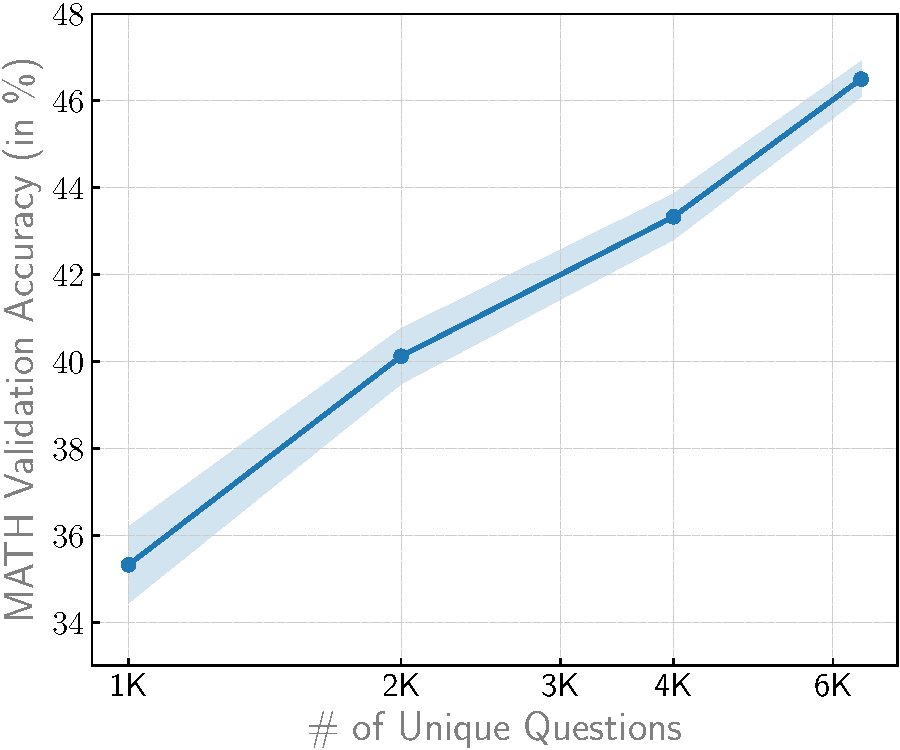
\includegraphics[width=0.85\linewidth]{plots/question_diversity.pdf}
    \caption{Impact of question diversity on MATH validation accuracy.} 
    \label{fig:question_diversity}
    \vspace{-0.2in}
\end{figure}
